\subsection*{Задача “Фактория”}

\subsubsection*{Задание}

Требуется разработать программу, имитирующую построение производственного конвейера в игровой форме с VR-интерфейсом.

Программа должна предоставлять пользователю возможности:
\begin{enumerate}
    \item Перемещаться по ограниченному игровому пространству размером 10x10 виртуальных метров с помощью комбинации “телепортации” и позиционирования.
    \item Загружать текущую сцену из файла input01.txt в текущем рабочем каталоге.
    \item Сохранять текущую сцену в файл output.txt в текущем рабочем каталоге.
    \item Переходить к следующему / предыдущему файлу в списке inputNN.txt, где NN -- число от 01 до 99.
    \item Отображать на сцене объекты следующих типов:
    \begin{enumerate}
        \item “Источник ресурсов” -- 4 вида, с различным визуальным отображением (деревья, минералы, $\dots$). Ограничивающий объём источника должен иметь форму параллелепипеда $1\times 1\times 1$ метра. 
        \item “Ресурсы и полуфабрикаты” 10 видов. Ограничивающий объем ресурса должен иметь форму куба со стороной 0,2 метра.
        \item “Конвейер” с указанным направлением движения, параллельным одной из осей X или Z. Ограничивающий объем конвейера должен иметь форму параллелепипеда $1\times 1\times 1$ метра.
        \item “Преобразователь/сборочный автомат” 10 видов, имеющих два входа и один выход. (принимает 2 ресурса и создает третий новый). Ограничивающий объем преобразователя должен иметь форму параллелепипеда 1x1x1 метра.
        \item “Склад” 1 вид, имеющий 4 входа. Ограничивающий объем склада должен иметь форму параллелепипеда $1\times 1\times 1$ метра    
    \end{enumerate}
    \item Выбирать тип создаваемых объектов.
    \item Создавать объекты текущего типа на сцене.
    \item Удалять и перемещать объекты на сцене при помощи контроллера.
    \item В момент завершения перемещения/создания объекта привязывать координаты объектов к сетке с шагом 0,1 метра. (округлять к меньшей координате сетки)
    \item Определять и визуально отображать присоединение концов конвейера к концам других конвейеров, входным и выходным портам преобразователей и источникам ресурсов. При этом присоединение по оси, перпендикулярной направлению конвейера, следует доводить до точного.
    \item Запускать и останавливать симуляцию. Визуально отображать её текущий статус.
    \item Запускать симуляцию на фиксированное количество секунд, указанное во входном файле.
    \item При запущенной симуляции:
    \begin{enumerate}
        \item Все ресурсы и полуфабрикаты, лежащие на конвейерах, перемещаются в направлении движения конвейера с равномерной скоростью 1 метр в секунду.
        \item Ресурсы появляются в геометрическом центре источника и двигаются в направлении каждого присоединенного конвейера. Для каждого конвейера появляется свой ресурс каждые 2 секунды. Если присоединено несколько конвейеров, то ресурс создается для каждого. (Первый ресурс появляется спустя 2 секунды после установки источника ресурса).
        \item Каждый ресурс появляется в геометрическом центре объекта и перемещается строго от геометрического центра одного объекта к геометрическому центру другого.                        
    \end{enumerate}
\end{enumerate}


Сборщик имеет буфер из ресурсов не того типа, который получается на выходе.
При достижении конца конвейерной ресурс падает на землю и исчезает.

Визуальное оформление должно:
\begin{enumerate}
    \item Включать пол, “skybox”, настроенную игровую зону, переключаемое отображение начала координат и координатных осей с рисками с шагом 1 метр.
    \item Позволять пользователю ясно различать все виды объектов на сцене, без усилий наблюдать за их движением.
    \item Иметь единое тематическое оформление в выбранной командой теме (“космос”, “первобытный мир”, “магия” и т.п.)        
\end{enumerate}

Художественный уровень оформления оценивается отдельно от технической работоспособности системы.	

\subsubsection*{Формат файла описания сцены}

Центр сцены находится в координатах (0, 0).

Файл содержит: (Все координаты -- 2D проекция на плоскость центра масс соответствующего объекта. Считать, что центр масс находится в центре масс соответствующего стереометрического однородного по плотности объекта).

\begin{itemize}
    \item Количество источников ресурсов
    
    Описание каждого объекта с новой строки. Координаты и номера ресурсов (0 - 3), каждый с новой строки.
    
    \item Количество видов преобразователей    
    
    Описание каждого объекта с новой строки. Координаты, два номера ресурсов (0 - 13) на входе и номер ресурса (4 - 13) на выходе.
    
    \item Количество конвейеров
    
    Описание каждого объекта с новой строки. Координаты, вектор направления.
    
    \item Количество складов
    
    Описание каждого объекта с новой строки. Координаты.
    
    \item Количество секунд симуляции или -1 (целое число), если симуляцию не нужно останавливать. После остановки симуляции необходимо сохранить объекты на сцене в файл output.txt и закрыть игру.        
\end{itemize}

Формат выходного файла
Количество ресурсов на сцене N целое число.
Последующие N строк содержат координаты ресурсов x, z и тип ресурсов.

Входной и выходной файл считывать и записывать из рабочей директории.

\subsubsection*{Схемы некоторых элементов сети}

\putImgWOCaption{16cm}{1}

\putImgWOCaption{16cm}{2}

\putImgWOCaption{16cm}{3}

\putImgWOCaption{16cm}{4}

\subsection*{Процесс работы над проектом}

Проект должен быть реализован в системе Unity.

Исходный код должен сохраняться в открытый git-репозиторий.

Push должен осуществляться не реже чем раз в полчаса.

Репозиторий должен содержать инструкции по сборке и пользовательскому интерфейсу. Проверка чек-поинтов и окончательная проверка осуществляется путем клонирования репозитория на компьютер жюри.


\subsubsection*{Пример входных/выходных файлов}

\begin{tabular}{|p{7cm}|p{7cm}|}
    \hline
    Входной файл & Выходной файл \\
    \hline
    \noindent{2

    4.5 4.5 0
    
    -2.5 2.5 1
    
    1
    
    1.5 1.5 0 1 4 0.0 1.0
    
    9
    
    3.5 4.5 1.0 0.0
    
    2.5 4.5 0.0 1.0
    
    2.5 3.5 0.0 1.0
    
    2.5 2.5 0.0 1.0
    
    2.5 1.5 1.0 0.0
    
    0.5 1.5 -1.0 0.0
    
    -0.5 1.5 -1.0 0.0
    
    -1.5 1.5 -1.0 0.0
    
    -2.5 1.5 -1.0 0.0
    
    1
    
    1.5 0.5
    
    10} &
    
    \noindent{8

    -2.5 2.48 1

    4.48 4.5 0

    1.5 1.4 4

    -1.48 1.5 1

    2.5 4.440001 0

    1.5 0.5000004 4

    0.5199993 1.5 1

    2.5 2.400001 0 } \\
    \hline
    \multicolumn{2}{|c|}{Визуализация}\\
    \hline
    \multicolumn{2}{|c|}{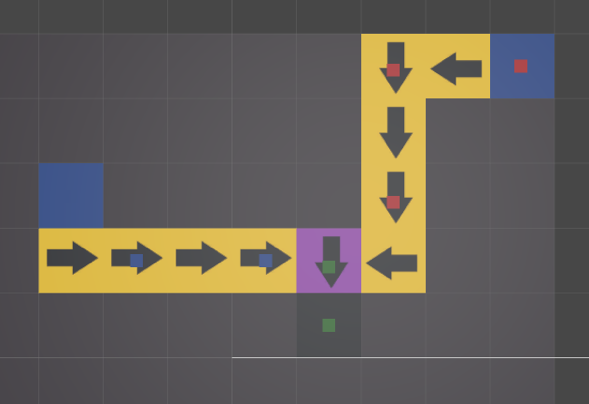
\includegraphics[height=5cm]{5}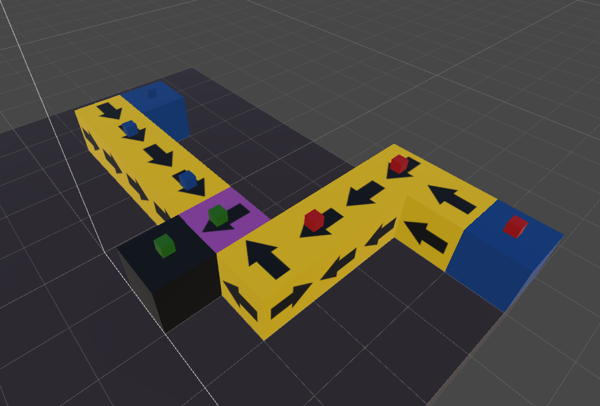
\includegraphics[height=5cm]{6}}\\
    
    \hline

\end{tabular}

\begin{tabular}{|p{7cm}|p{7cm}|}
    \hline
    \textbf{Входной файл} & \textbf{Выходной файл} \\
    \hline
    \noindent{3

    -2.5 -2.5 2

    -1.5 0.5 1

    -1.5 2.5 0

    2

    0.5 0.5 0 4 5 -1.0 0.0

    -1.5 -1.5 1 2 4 -1.0 0.0

    11

    1.5 0.5 -1.0 0.0

    0.5 -0.5 0.0 -1.0

    0.5 -1.5 0.0 -1.0

    -0.5 -1.5 -1.0 0.0

    -1.5 -2.5 0.0 -1.0

    -1.5 -0.5 0.0 1.0

    0.5 1.5 0.0 1.0

    0.5 2.5 0.0 1.0

    0.5 3.5 0.0 1.0

    -0.5 3.5 -1.0 0.0

    -1.5 3.5 -1.0 0.0

    1

    2.5 0.5

    11 } &
    \noindent{9

    -0.5 -1.5 4

    1.5 0.5 5

    -1.5 3.5 0

    -1.5 -0.5 1

    -1.5 -2.5 2

    0.5 -0.5 4

    2.5 0.5 5

    0.5 3.5 0

    0.5 1.5 0 } \\
    \hline
    \multicolumn{2}{|c|}{\textbf{Визуализация}}\\
    \hline
    \multicolumn{2}{|c|}{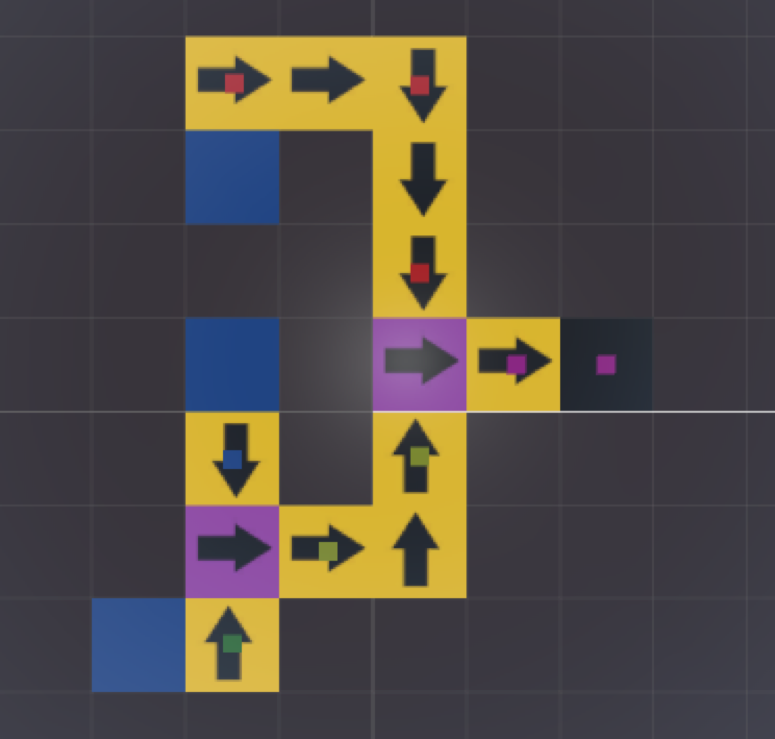
\includegraphics[height=5.5cm]{7}}\\
    
    \hline

\end{tabular}

\begin{tabular}{|p{7cm}|p{7cm}|}
    \hline
    \textbf{Входной файл} & \textbf{Выходной файл} \\
    \hline
    \noindent{2
    0.5 4.5 0

    -1.5 3.5 1

    1

    -0.5 -0.5 0 1 4 -1.0 0.0

    5

    -0.5 4.5 0.0 1.0

    -0.5 3.5 0.0 1.0

    -0.5 2.5 0.0 1.0

    -0.5 1.5 0.0 1.0

    -0.5 0.5 0.0 1.0

    1

    0.5 -0.5

    9 } &
    
    \noindent{7

    -0.5 3.5 1

    -0.5 4.5 0

    0.5 -0.5 4

    -0.5 1.5 1

    -0.5 2.5 0

    -0.5 -0.5 1

    -0.5 0.5 0
     } \\
    \hline
    \multicolumn{2}{|c|}{\textbf{Визуализация}}\\
    \hline
    \multicolumn{2}{|c|}{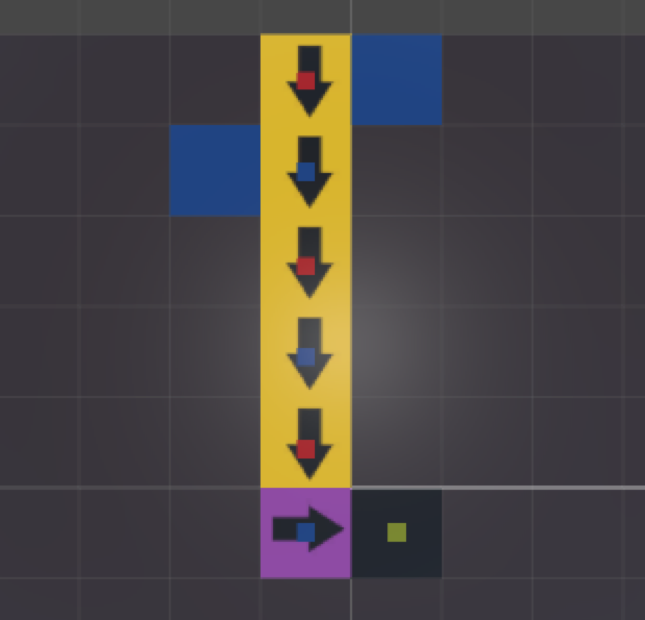
\includegraphics[height=5.5cm]{8}}\\
    
    \hline

\end{tabular}
